\section{Register description}
\regover{
{\hyperref[pdm-audpdm-top]{audpdm\_top}}&
\\
\hline
{\hyperref[pdm-audpdm-itf]{audpdm\_itf}}&
\\
\hline
{\hyperref[pdm-pdm-adc-0]{pdm\_adc\_0}}&
\\
\hline
{\hyperref[pdm-pdm-adc-1]{pdm\_adc\_1}}&
\\
\hline
{\hyperref[pdm-pdm-dac-0]{pdm\_dac\_0}}&
\\
\hline
{\hyperref[pdm-pdm-pdm-0]{pdm\_pdm\_0}}&
\\
\hline
{\hyperref[pdm-pdm-rsvd0]{pdm\_rsvd0}}&
\\
\hline
{\hyperref[pdm-pdm-dbg-0]{pdm\_dbg\_0}}&
\\
\hline
{\hyperref[pdm-pdm-dbg-1]{pdm\_dbg\_1}}&
\\
\hline
{\hyperref[pdm-pdm-dbg-2]{pdm\_dbg\_2}}&
\\
\hline
{\hyperref[pdm-pdm-dbg-3]{pdm\_dbg\_3}}&
\\
\hline
{\hyperref[pdm-pdm-dbg-4]{pdm\_dbg\_4}}&
\\
\hline
{\hyperref[pdm-pdm-adc-s0]{pdm\_adc\_s0}}&
\\
\hline
{\hyperref[pdm-pdm-adc-s1]{pdm\_adc\_s1}}&
\\
\hline
{\hyperref[pdm-pdm-adc-s2]{pdm\_adc\_s2}}&
\\
\hline
{\hyperref[pdm-pdm-rx-fifo-ctrl]{pdm\_rx\_fifo\_ctrl}}&
\\
\hline
{\hyperref[pdm-pdm-rx-fifo-status]{pdm\_rx\_fifo\_status}}&
\\
\hline
{\hyperref[pdm-pdm-rx-fifo-data]{pdm\_rx\_fifo\_data}}&
\\
\hline
}

\subsection{audpdm\_top}
\label{pdm-audpdm-top}
Address:0x2000ac00
 \begin{figure}[H]
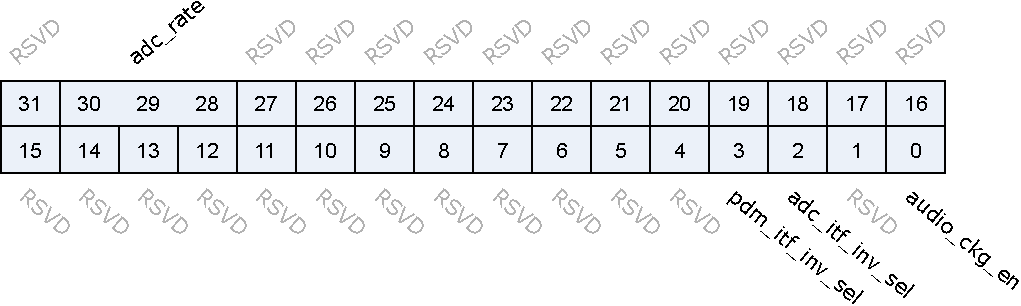
\includegraphics{pdm_audpdm_top.pdf}
\end{figure}

\regdes{31&RSVD& & & \\\hline
30:28&adc\_rate&r/w&3'd1&adc fs 0:8kHz,1:16kHz, 2:24kHz(22.05k), 3:32kHz, 4:48kHz(44.1k), 5:96kHz, 6:reserved, 7:manual\\\hline
27&RSVD& & & \\\hline
26:24&dac\_rate&r/w&3'd4&dac fs 0:8kHz,1:16kHz, 2:24kHz(22.05k), 3:32kHz, 4:48kHz(44.1k), 5:96kHz, 6:192kHz, 7:manual\\\hline
23:4&RSVD& & & \\\hline
3&pdm\_itf\_inv\_sel&r/w&1'd0&1:invert clk\_pdm\_inf\\\hline
2&adc\_itf\_inv\_sel&r/w&1'd0&1:invert clk\_adc\_itf\\\hline
1&dac\_itf\_inv\_sel&r/w&1'd1&1:invert clk\_dac\_itf\\\hline
0&audio\_ckg\_en&r/w&1'd0&1:enable audio clock generator\\\hline

}
\subsection{audpdm\_itf}
\label{pdm-audpdm-itf}
Address:0x2000ac04
 \begin{figure}[H]
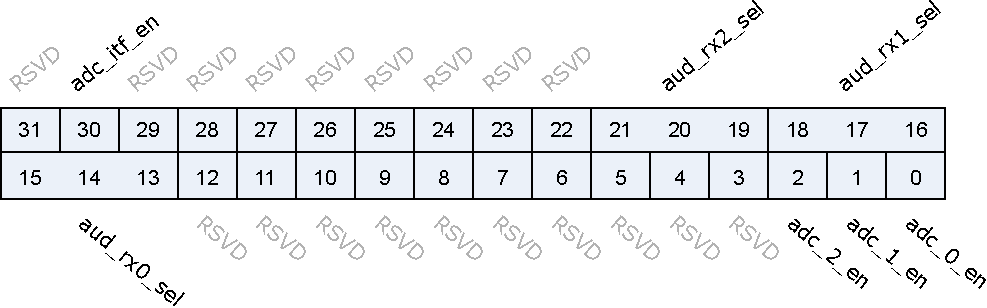
\includegraphics{pdm_audpdm_itf.pdf}
\end{figure}

\regdes{31&dac\_itf\_en&r/w&1'd0&1:enable dac to audio dma interface\\\hline
30&adc\_itf\_en&r/w&1'd0&1:enable adc to audio dma interface\\\hline
29&aud\_tx1\_sel&r/w&1'd1&audio tx1 source select; 0:dac ch0, 1:dac ch1\\\hline
28&aud\_tx0\_sel&r/w&1'd0&audio tx0 source select; 0:dac ch0, 1:dac ch1\\\hline
27:25&aud\_rx4\_sel&r/w&3'd4&audio rx4 source select; 0:adc ch0, 1:adc ch1, 2:adc ch2, 3:aec ch0, 4:aec ch1\\\hline
24:22&aud\_rx3\_sel&r/w&3'd3&audio rx3 source select; 0:adc ch0, 1:adc ch1, 2:adc ch2, 3:aec ch0, 4:aec ch1\\\hline
21:19&aud\_rx2\_sel&r/w&3'd2&audio rx2 source select; 0:adc ch0, 1:adc ch1, 2:adc ch2, 3:aec ch0, 4:aec ch1\\\hline
18:16&aud\_rx1\_sel&r/w&3'd1&audio rx1 source select; 0:adc ch0, 1:adc ch1, 2:adc ch2, 3:aec ch0, 4:aec ch1\\\hline
15:13&aud\_rx0\_sel&r/w&3'd0&audio rx0 source select; 0:adc ch0, 1:adc ch1, 2:adc ch2, 3:aec ch0, 4:aec ch1\\\hline
12:7&RSVD& & & \\\hline
6&aec\_1\_en&r/w&1'd0&1:enable aec ch1\\\hline
5&aec\_0\_en&r/w&1'd0&1:enable aec ch0\\\hline
4&dac\_1\_en&r/w&1'd0&1:enable dac ch1\\\hline
3&dac\_0\_en&r/w&1'd0&1:enable dac ch0\\\hline
2&adc\_2\_en&r/w&1'd0&1:enable adc ch2\\\hline
1&adc\_1\_en&r/w&1'd0&1:enable adc ch1\\\hline
0&adc\_0\_en&r/w&1'd0&1:enable adc ch0\\\hline

}
\subsection{pdm\_adc\_0}
\label{pdm-pdm-adc-0}
Address:0x2000ac08
 \begin{figure}[H]
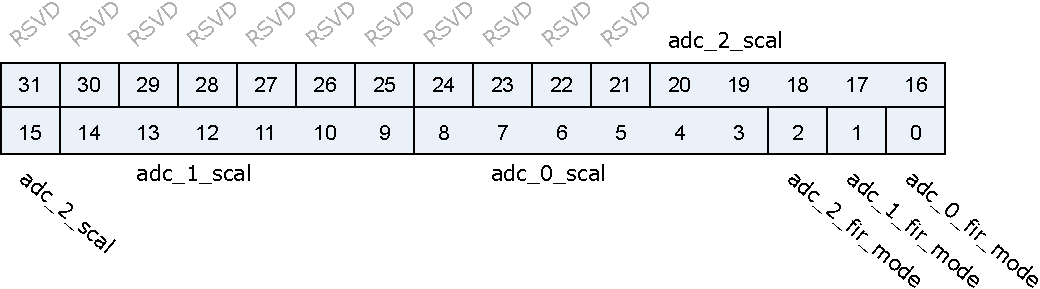
\includegraphics{pdm_pdm_adc_0.pdf}
\end{figure}

\regdes{31:30&adc\_lfsr\_mode&r/w&2'd0&0:LFSR32, 1:LFSR24, 2:LFSR16, 3:LFSR12\\\hline
29&adc\_dither\_data&r&1'd1&read LFSR out\\\hline
28:21&RSVD& & & \\\hline
20:15&adc\_2\_scal&r/w&6'd32&adc ch2 scaling value; u6.5\\\hline
14:9&adc\_1\_scal&r/w&6'd32&adc ch1 scaling value; u6.5\\\hline
8:3&adc\_0\_scal&r/w&6'd32&adc ch0 scaling value; u6.5\\\hline
2&adc\_2\_fir\_mode&r/w&1'd0&adc fir mode\\\hline
1&adc\_1\_fir\_mode&r/w&1'd0&adc fir mode\\\hline
0&adc\_0\_fir\_mode&r/w&1'd0&adc fir mode\\\hline

}
\subsection{pdm\_adc\_1}
\label{pdm-pdm-adc-1}
Address:0x2000ac0c
 \begin{figure}[H]
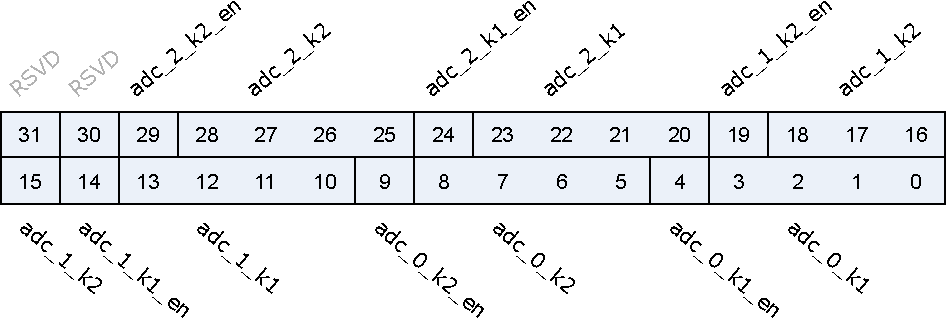
\includegraphics{pdm_pdm_adc_1.pdf}
\end{figure}

\regdes{31:30&RSVD& & & \\\hline
29&adc\_2\_k2\_en&r/w&1'd0&adc ch2 hpf parameter k2 enable\\\hline
28:25&adc\_2\_k2&r/w&4'd13&adc ch2 hpf parameter k2\\\hline
24&adc\_2\_k1\_en&r/w&1'd1&adc ch2 hpf parameter k1 enable\\\hline
23:20&adc\_2\_k1&r/w&4'd8&adc ch2 hpf parameter k1\\\hline
19&adc\_1\_k2\_en&r/w&1'd0&adc ch1 hpf parameter k2 enable\\\hline
18:15&adc\_1\_k2&r/w&4'd13&adc ch1 hpf parameter k2\\\hline
14&adc\_1\_k1\_en&r/w&1'd1&adc ch1 hpf parameter k1 enable\\\hline
13:10&adc\_1\_k1&r/w&4'd8&adc ch1 hpf parameter k1\\\hline
9&adc\_0\_k2\_en&r/w&1'd0&adc ch0 hpf parameter k2 enable\\\hline
8:5&adc\_0\_k2&r/w&4'd13&adc ch0 hpf parameter k2\\\hline
4&adc\_0\_k1\_en&r/w&1'd1&adc ch0 hpf parameter k1 enable\\\hline
3:0&adc\_0\_k1&r/w&4'd8&adc ch0 hpf parameter k1\\\hline

}
\subsection{pdm\_dac\_0}
\label{pdm-pdm-dac-0}
Address:0x2000ac10
 \begin{figure}[H]
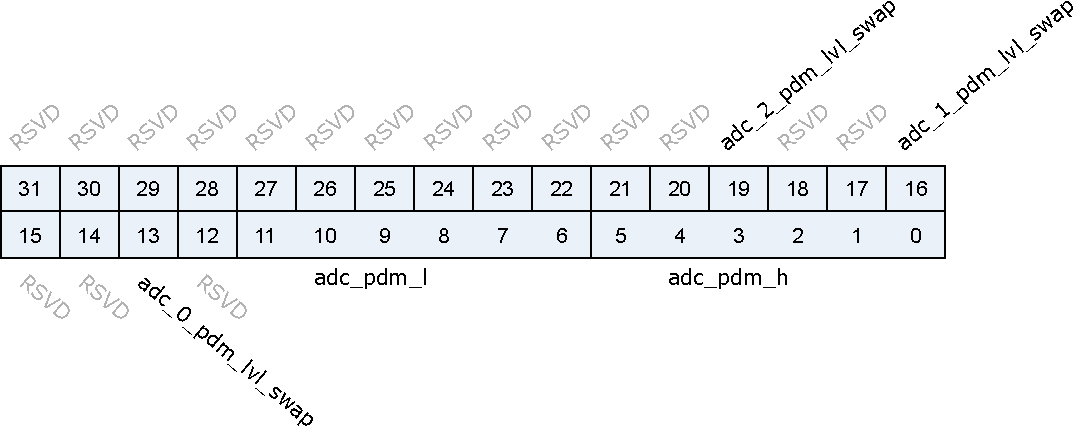
\includegraphics{pdm_pdm_dac_0.pdf}
\end{figure}

\regdes{31&RSVD& & & \\\hline
30:28&mix\_0\_att\_mode2&r/w&3'd0&0: 0db,1:6db, 2:12db, 3:18db, 4:36db, 5:54db, 6:72db, 7:mute\\\hline
27:25&mix\_0\_att\_mode1&r/w&3'd0&0: 0db,1:6db, 2:12db, 3:18db, 4:36db, 5:54db, 6:72db, 7:mute\\\hline
24:23&mix\_0\_mode&r/w&2'd0&0: no mix, 1: mix second input, 2: mix sidetone/loopback\\\hline
22:21&mix\_0\_sel&r/w&2'd0&0: 0, 1:adc ch0, 2: adc ch1, 3:adc ch2\\\hline
20&adc\_2\_mash\_bit\_swap&r/w&1'd0&1:swap adc1\_do1 and adc1\_do2\\\hline
19&adc\_2\_pdm\_lvl\_swap&r/w&1'd0&1:invert pdm input data\\\hline
18&adc\_2\_src&r/w&1'd0&0:adc, 1:pdm\\\hline
17&adc\_1\_mash\_bit\_swap&r/w&1'd0&1:swap adc2\_do1 and adc2\_do2\\\hline
16&adc\_1\_pdm\_lvl\_swap&r/w&1'd0&1:invert pdm input data\\\hline
15&adc\_1\_src&r/w&1'd0&0:adc, 1:pdm\\\hline
14&adc\_0\_mash\_bit\_swap&r/w&1'd0&1:swap adc3\_do1 and adc3\_do2\\\hline
13&adc\_0\_pdm\_lvl\_swap&r/w&1'd0&1:invert pdm input data\\\hline
12&adc\_0\_src&r/w&1'd0&0:adc, 1:pdm\\\hline
11:6&adc\_pdm\_l&r/w&6'h3f&pdm low value\\\hline
5:0&adc\_pdm\_h&r/w&6'h1&pdm high value\\\hline
-1:31&RSVD& & & \\\hline
30:28&mix\_1\_att\_mode2&r/w&3'd0&0: 0db,1:6db, 2:12db, 3:18db, 4:36db, 5:54db, 6:72db, 7:mute\\\hline
27:25&mix\_1\_att\_mode1&r/w&3'd0&0: 0db,1:6db, 2:12db, 3:18db, 4:36db, 5:54db, 6:72db, 7:mute\\\hline
24:23&mix\_1\_mode&r/w&2'd0&0: no mix, 1: mix second input, 2: mix sidetone/loopback\\\hline
22:21&mix\_1\_sel&r/w&2'd0&0: 0, 1:adc ch0, 2: adc ch1, 3:adc ch2\\\hline
20:17&RSVD& & & \\\hline
16:15&dac\_dsm\_dither\_prbs\_mode&r/w&1'd0&dac dsm dither lfsr mode:0:LFSR32, 1:LFSR24, 2:LFSR16, 3:LFSR12\\\hline
14&dac\_dsm\_dither\_en&r/w&1'd1&1:enable dac dsm dither\\\hline
13:11&dac\_dsm\_dither\_amp&r/w&3'd0&dac dsm dither amplitue\\\hline
10&dac\_dsm\_scaling\_en&r/w&1'd1&1:enable dac dsm scaling\\\hline
9:6&dac\_dsm\_scaling\_factor&r/w&4'd15&dac dsm scaling value;  u4.4\\\hline
5&dac\_dsm\_order&r/w&1'd0&0: 2-order, 1: 3-order\\\hline
4:2&RSVD& & & \\\hline
1&dac\_dem\_out\_swap&r/w&1'd0&1:swap dacldata and dacrdata\\\hline
0&dac\_dem\_bypass&r/w&1'd0&1:bypass dac dwa\\\hline
-1:14&RSVD& & & \\\hline
13&aec\_record\_vld\_4s\_en&r/w&1'd0&0:aec record vld auto controlled by dac\_rate, 1:enable aec record vld manual mode\\\hline
12:11&aec\_record\_vld\_4s\_div&r/w&2'd0&aec record vld manual divide rate\\\hline
10:8&aec\_1\_atten\_mode&r/w&3'd0&aec ch1 attenuation mode: 0:no attenuation, 1:drop 1LSB, 2:drop 2LSB, 3:drop 3LSB, 4:drop 6LSB, 5:drop 9LSB, 6:drop 12LSB\\\hline
7:5&aec\_0\_atten\_mode&r/w&3'd0&aec ch0 attenuation mode: 0:no attenuation, 1:drop 1LSB, 2:drop 2LSB, 3:drop 3LSB, 4:drop 6LSB, 5:drop 9LSB, 6:drop 12LSB\\\hline
4:0&RSVD& & & \\\hline

}
\subsection{pdm\_pdm\_0}
\label{pdm-pdm-pdm-0}
Address:0x2000ac1c
 \begin{figure}[H]
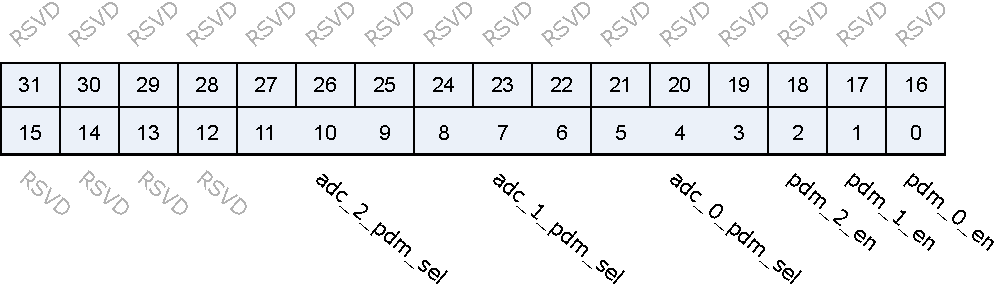
\includegraphics{pdm_pdm_pdm_0.pdf}
\end{figure}

\regdes{31:12&RSVD& & & \\\hline
11:9&adc\_2\_pdm\_sel&r/w&3'd2&adc ch2 source select: 0:pdm\_0\_l, 1:pdm\_0\_r, 2:pdm\_1\_l, 3:pdm\_1\_r, 4:pdm\_2\_l, 5:pdm\_2\_r\\\hline
8:6&adc\_1\_pdm\_sel&r/w&3'd1&adc ch1 source select: 0:pdm\_0\_l, 1:pdm\_0\_r, 2:pdm\_1\_l, 3:pdm\_1\_r, 4:pdm\_2\_l, 5:pdm\_2\_r\\\hline
5:3&adc\_0\_pdm\_sel&r/w&3'd0&adc ch0 source select: 0:pdm\_0\_l, 1:pdm\_0\_r, 2:pdm\_1\_l, 3:pdm\_1\_r, 4:pdm\_2\_l, 5:pdm\_2\_r\\\hline
2&pdm\_2\_en&r/w&1'd0&1:enable pdm\_2\\\hline
1&pdm\_1\_en&r/w&1'd0&1:enable pdm\_1\\\hline
0&pdm\_0\_en&r/w&1'd0&1:enable pdm\_0\\\hline

}
\subsection{pdm\_rsvd0}
\label{pdm-pdm-rsvd0}
Address:0x2000ac20
 \begin{figure}[H]
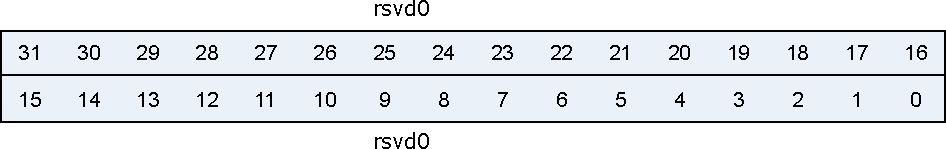
\includegraphics{pdm_pdm_rsvd0.pdf}
\end{figure}

\regdes{31:0&rsvd0&r/w&32'hffff&\\\hline

}
\subsection{pdm\_dbg\_0}
\label{pdm-pdm-dbg-0}
Address:0x2000ac24
 \begin{figure}[H]
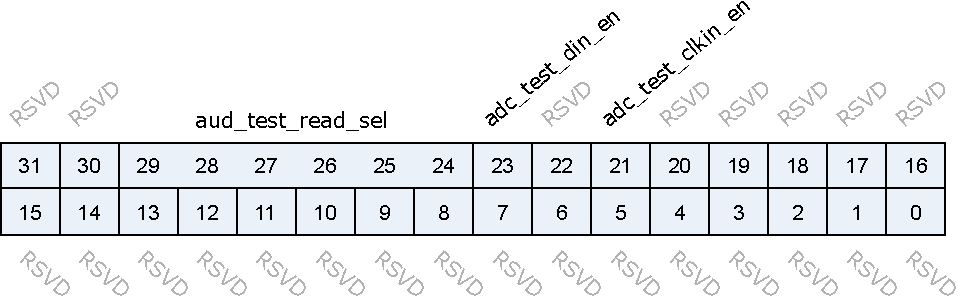
\includegraphics{pdm_pdm_dbg_0.pdf}
\end{figure}

\regdes{31:30&RSVD& & & \\\hline
29:24&aud\_test\_read\_sel&r/w&6'd0&select aud\_test\_read(0x28) test point\\\hline
23&adc\_test\_din\_en&r/w&1'd0&1:enable adc test data input from GPIO\\\hline
22&dac\_test\_din\_en&r/w&1'd0&1:enable dac test data input from GPIO\\\hline
21&adc\_test\_clkin\_en&r/w&1'd0&1:enable adc test clcok input from GPIO\\\hline
20&dac\_test\_clkin\_en&r/w&1'd0&1:enable dac test clcok input from GPIO\\\hline
19:18&audio\_test\_out\_sel&r/w&2'd0&audio test data to GPIO select: 0:no data, 1:adc ch0/1/2, 2:dac ch0 dwa, 2:dac ch1 dwa\\\hline
17:4&RSVD& & & \\\hline
3:1&aud\_sin\_step&r/w&3'd2&step of dac audio sin table @FS=192k \par 0:div1, 1:div2, 2:div4, 3:div6, 4:div8, 5:div12, 6:div24
\\\hline
0&aud\_sin\_en&r/w&1'd0&1:enable audio dac sin generator\\\hline

}
\subsection{pdm\_dbg\_1}
\label{pdm-pdm-dbg-1}
Address:0x2000ac28
 \begin{figure}[H]
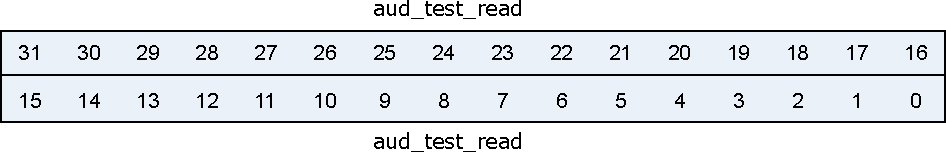
\includegraphics{pdm_pdm_dbg_1.pdf}
\end{figure}

\regdes{31:0&aud\_test\_read&r&32'd0&audio test read value\\\hline

}
\subsection{pdm\_dbg\_2}
\label{pdm-pdm-dbg-2}
Address:0x2000ac2c
 \begin{figure}[H]
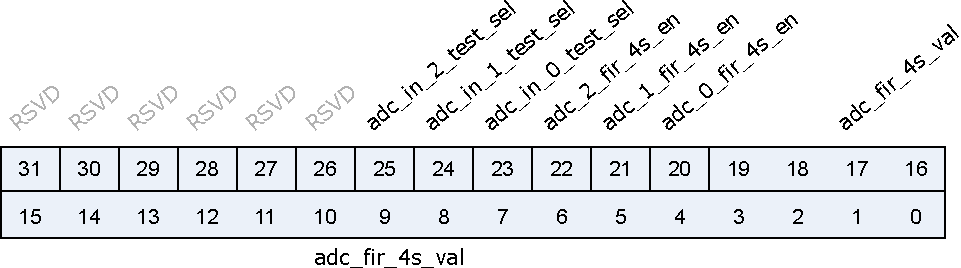
\includegraphics{pdm_pdm_dbg_2.pdf}
\end{figure}

\regdes{31:26&RSVD& & & \\\hline
25&adc\_in\_2\_test\_sel&r/w&1'd0&adc ch2 test data select; 1:from adc sin generator, 0:from fir force value \\\hline
24&adc\_in\_1\_test\_sel&r/w&1'd0&adc ch1 test data select; 1:from adc sin generator, 0:from fir force value \\\hline
23&adc\_in\_0\_test\_sel&r/w&1'd0&adc ch0 test data select; 1:from adc sin generator, 0:from fir force value \\\hline
22&adc\_2\_fir\_4s\_en&r/w&1'd0&1:force adc ch2 fir output\\\hline
21&adc\_1\_fir\_4s\_en&r/w&1'd0&1:force adc ch1 fir output\\\hline
20&adc\_0\_fir\_4s\_en&r/w&1'd0&1:force adc ch0 fir output\\\hline
19:0&adc\_fir\_4s\_val&r/w&20'd0&force value of adc fir output \\\hline

}
\subsection{pdm\_dbg\_3}
\label{pdm-pdm-dbg-3}
Address:0x2000ac30
 \begin{figure}[H]
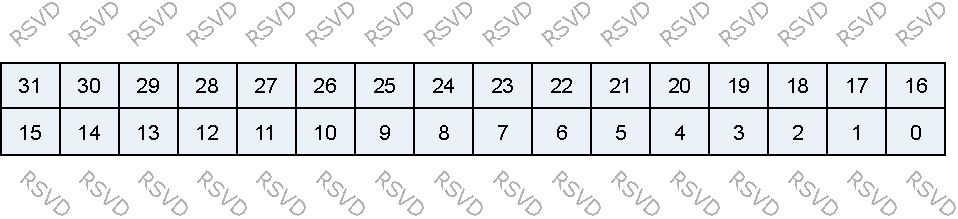
\includegraphics{pdm_pdm_dbg_3.pdf}
\end{figure}

\regdes{31:24&RSVD& & & \\\hline
23&dac\_in\_1\_test\_sel&r/w&1'd0&dac ch1 test data select; 0:from dac sin generator, 1:from dac force value\\\hline
22&dac\_in\_0\_test\_sel&r/w&1'd0&dac ch0 test data select; 0:from dac sin generator, 1:from dac force value\\\hline
21&dac\_dwa\_1\_4s\_en&r/w&1'd0&1:force dac ch1 dwa data from dac\_4s\_val[6:0]\\\hline
20&dac\_dwa\_0\_4s\_en&r/w&1'd0&1:force dac ch0 dwa data from dac\_4s\_val[6:0]\\\hline
19:0&dac\_4s\_val&r/w&20'd0&dac force value\\\hline

}
\subsection{pdm\_dbg\_4}
\label{pdm-pdm-dbg-4}
Address:0x2000ac34
 \begin{figure}[H]
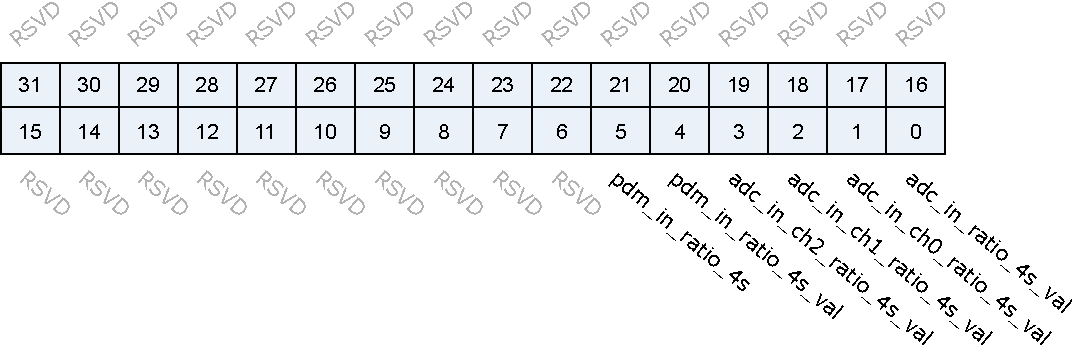
\includegraphics{pdm_pdm_dbg_4.pdf}
\end{figure}

\regdes{31:11&RSVD& & & \\\hline
10:8&aec\_fs\_rate\_4s\_val&r/w&3'd0&\\\hline
7:6&dac\_out\_ratio\_4s\_val&r/w&2'd0&\\\hline
5&pdm\_in\_ratio\_4s&r/w&1'd0&\\\hline
4&pdm\_in\_ratio\_4s\_val&r/w&1'd0&\\\hline
3&adc\_in\_ch2\_ratio\_4s\_val&r/w&1'd0&\\\hline
2&adc\_in\_ch1\_ratio\_4s\_val&r/w&1'd0&\\\hline
1&adc\_in\_ch0\_ratio\_4s\_val&r/w&1'd0&\\\hline
0&adc\_in\_ratio\_4s\_val&r/w&1'd0&\\\hline

}
\subsection{pdm\_adc\_s0}
\label{pdm-pdm-adc-s0}
Address:0x2000ac38
 \begin{figure}[H]
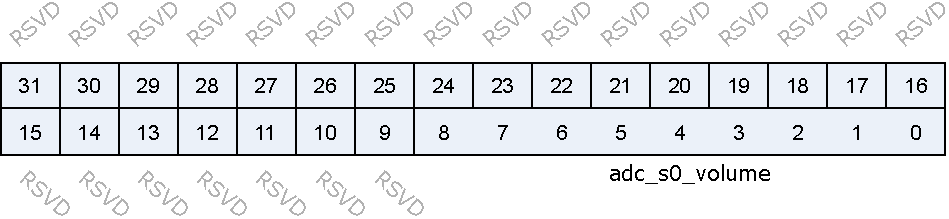
\includegraphics{pdm_pdm_adc_s0.pdf}
\end{figure}

\regdes{31:9&RSVD& & & \\\hline
8:0&adc\_s0\_volume&r/w&9'd0&volume s9.1, -95.5dB ~ +18dB in 0.5dB step\\\hline

}
\subsection{pdm\_adc\_s1}
\label{pdm-pdm-adc-s1}
Address:0x2000ac3c
 \begin{figure}[H]
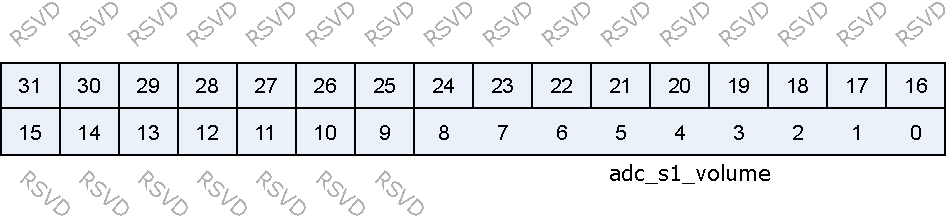
\includegraphics{pdm_pdm_adc_s1.pdf}
\end{figure}

\regdes{31:9&RSVD& & & \\\hline
8:0&adc\_s1\_volume&r/w&9'd0&volume s9.1, -95.5dB ~ +18dB in 0.5dB step\\\hline

}
\subsection{pdm\_adc\_s2}
\label{pdm-pdm-adc-s2}
Address:0x2000ac40
 \begin{figure}[H]
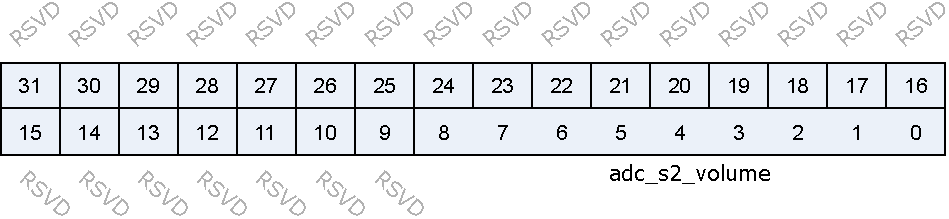
\includegraphics{pdm_pdm_adc_s2.pdf}
\end{figure}

\regdes{31:9&RSVD& & & \\\hline
8:0&adc\_s2\_volume&r/w&9'd0&volume s9.1, -95.5dB ~ +18dB in 0.5dB step\\\hline

}
\subsection{pdm\_rx\_fifo\_ctrl}
\label{pdm-pdm-rx-fifo-ctrl}
Address:0x2000ac80
 \begin{figure}[H]
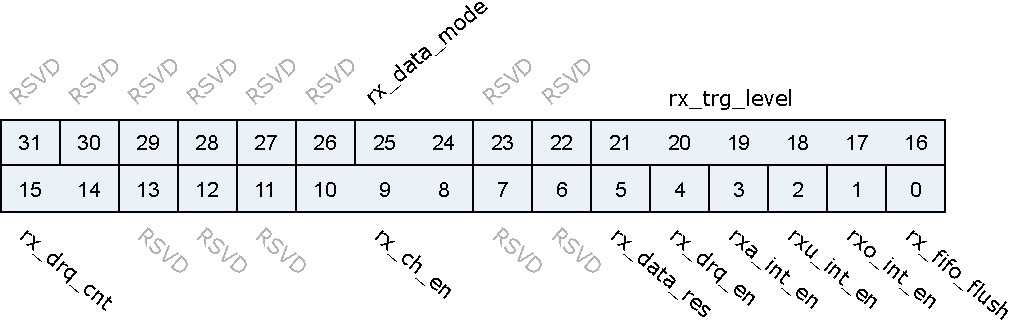
\includegraphics{pdm_pdm_rx_fifo_ctrl.pdf}
\end{figure}

\regdes{31:26&RSVD& & & \\\hline
25:24&rx\_data\_mode&r/w&2'b0&RX\_FIFO\_DATOUT\_MODE. \par RX FIFO DATA Output Mode (Mode 0, 1, 2, 3) \par Mode 0: Valid data's MSB is at [31] of RX\_FIFO register \par Mode 1: Valid data's MSB is at [23] of RX\_FIFO register \par Mode 2: Valid data's MSB is at [19] of RX\_FIFO register \par Mode 3: Valid data's MSB is at [15] of RX\_FIFO register \par Note: Expanding ‘0’ at LSB of RX FIFO register (data invalid region) \par            Expanding sign bit at MSB of RX FIFO register (data invalid region) \par For 20-bit received audio sample resolution: \par Mode 0: RXDATA[31:0] = {FIFO\_O[19:0], 12’h0} \par Mode 1: RXDATA[31:0] = {8{FIFO\_O[19]}, FIFO\_O[19:0], 4’h0} \par Mode 2: RXDATA[31:0] = {12{FIFO\_O[19]}, FIFO\_O[19:0]} \par Mode 3: RXDATA[31:0] = {16{FIFO\_O[19]}, FIFO\_O[19:4]} \par For 16-bit received audio sample resolution: \par Mode 0: RXDATA[31:0] = {FIFO\_O[19:4], 16’h0} \par Mode 1: RXDATA[31:0] = {8{FIFO\_O[19]}, FIFO\_O[19:4], 8’h0} \par Mode 2: RXDATA[31:0] = {12{FIFO\_O[19]}, FIFO\_O[19:4], 4'h0} \par Mode 3: RXDATA[31:0] = {16{FIFO\_O[19]}, FIFO\_O[19:4]}
\\\hline
23:22&RSVD& & & \\\hline
21:16&rx\_trg\_level&r/w&6'd23&RX\_FIFO\_TRG\_LEVEL. \par RX FIFO Trigger Level (RXTL[5:0]) \par Interrupt and DMA request trigger level for RX FIFO Data Available condition \par IRQ/DRQ Generated when WLEVEL > RXTL[5:0] \par Notes: \par WLEVEL represents the number of valid samples in the RX FIFO
\\\hline
15:14&rx\_drq\_cnt&r/w&2'b0&RX\_DRQ\_CLR\_CNT. \par When RX FIFO available data less than or equal N, DRQ Request will be de-asserted. N is defined here: \par 00: IRQ/DRQ de-asserted when WLEVEL <= RXTL[5:0] \par 01: IRQ/DRQ de-asserted when WLEVEL < 8 \par 10: IRQ/DRQ de-asserted when WLEVEL < 16 \par 11: IRQ/DRQ de-asserted when WLEVEL < 32 \par WLEVEL represents the number of valid samples in the RX FIFO
\\\hline
13:11&RSVD& & & \\\hline
10:8&rx\_ch\_en&r/w&3'b0&RX\_FIFO\_DATIN\_SRC. \par RX FIFO Data Input Source Select. \par 0: Disable 1: Enable \par Bit10: ADC3 data \par Bit9: ADC2 data \par Bit8: ADC1 data \par When some of the above bits set to ’1’, these data are always arranged in order from low-bit to high-bit.(bit8->bit10)
\\\hline
7:6&RSVD& & & \\\hline
5&rx\_data\_res&r/w&1'b0&RX\_SAMPLE\_BITS. \par Receiving Audio Sample Resolution \par 0: 16 bits \par 1: 20 bits
\\\hline
4&rx\_drq\_en&r/w&1'b0&ADC\_DRQ\_EN. \par ADC FIFO Data Available DRQ Enable. \par 0: Disable \par 1: Enable
\\\hline
3&rxa\_int\_en&r/w&1'b0&ADC\_IRQ\_EN. \par ADC FIFO Data Available IRQ Enable. \par 0: Disable \par 1: Enable
\\\hline
2&rxu\_int\_en&r/w&1'b0&ADC\_UNDERRUN\_IRQ\_EN. \par ADC FIFO Under Run IRQ Enable \par 0: Disable \par 1: Enable
\\\hline
1&rxo\_int\_en&r/w&1'b0&ADC\_OVERRUN\_IRQ\_EN. \par ADC FIFO Over Run IRQ Enable \par 0: Disable \par 1: Enable
\\\hline
0&rx\_fifo\_flush&w1c&1'b0&ADC\_FIFO\_FLUSH. \par ADC FIFO Flush. \par Write ‘1’ to flush TX FIFO, self clear to ‘0’.
\\\hline

}
\subsection{pdm\_rx\_fifo\_status}
\label{pdm-pdm-rx-fifo-status}
Address:0x2000ac84
 \begin{figure}[H]
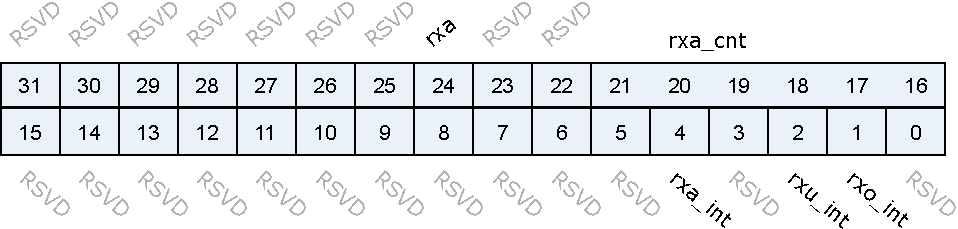
\includegraphics{pdm_pdm_rx_fifo_status.pdf}
\end{figure}

\regdes{31:25&RSVD& & & \\\hline
24&rxa&r&1'b0&RXA. \par RX FIFO Available \par 0: No available data in RX FIFO \par 1: More than one sample in RX FIFO (>= 1 word)
\\\hline
23:22&RSVD& & & \\\hline
21:16&rxa\_cnt&r&6'h0&RXA\_CNT. \par RX FIFO Available Sample Word Counter
\\\hline
15:5&RSVD& & & \\\hline
4&rxa\_int&r&1'b0&RXA\_INT. \par RX FIFO Data Available Pending Interrupt \par 0: No Pending IRQ \par 1: Data Available Pending IRQ \par Automatic clear if interrupt condition fails.
\\\hline
3&RSVD& & & \\\hline
2&rxu\_int&r&1'b0&RXU\_INT. \par RX FIFO Underrun Pending Interrupt \par 0: No Pending IRQ \par 1: FIFO Underrun Pending IRQ \par Write ‘1’ to clear this interrupt
\\\hline
1&rxo\_int&r&1'b0&RXO\_INT. \par RX FIFO Overrun Pending Interrupt \par 0: No Pending IRQ \par 1: FIFO Overrun Pending IRQ \par Write ‘1’ to clear this interrupt
\\\hline
0&RSVD& & & \\\hline

}
\subsection{pdm\_rx\_fifo\_data}
\label{pdm-pdm-rx-fifo-data}
Address:0x2000ac88
 \begin{figure}[H]
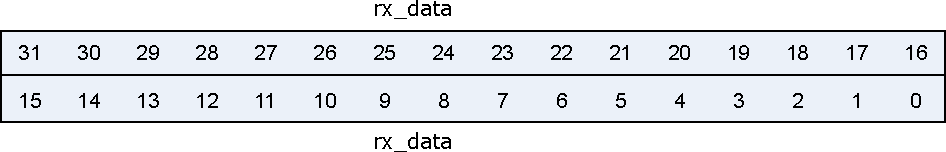
\includegraphics{pdm_pdm_rx_fifo_data.pdf}
\end{figure}

\regdes{31:0&rx\_data&r&32'h0&RX\_DATA. \par RX Sample \par Host can get one sample by reading this register. The left channel sample data is first and then the right channel sample.
\\\hline

}
